\documentclass{beamer}

\usepackage[utf8]{inputenc}
\usecolortheme{beaver}
\usepackage{caption}
\usepackage{subcaption}
\usepackage{mathtools}
\usepackage{todonotes}
\usepackage{amsmath}
\usepackage{bm}
\usepackage{listings}
\usepackage{ragged2e}
\usepackage{titlecaps}
\usepackage{fancyvrb}
\def\ci{\perp\!\!\!\!\!\perp}

\newtheorem{proposition}{Proposition}
\Addlcwords{for a is but and with of in as the etc on to if}

\newcommand\github{
\includegraphics[height=2ex]{imgs/github.png}}
\newcommand\email{
\includegraphics[height=3ex]{imgs/email.png}}

\setbeamertemplate{section in toc}{\inserttocsectionnumber.~\inserttocsection}
\usetheme{Boadilla}
\makeatletter
\setbeamertemplate{footline}{%
    \leavevmode%
    \hbox{%
        \begin{beamercolorbox}[wd=.3\paperwidth,ht=2.25ex,dp=1ex,center]{author in head/foot}%
            \usebeamerfont{author in head/foot}\insertshortauthor\expandafter\beamer@ifempty\expandafter{\beamer@shortinstitute}{}{~~(\insertshortinstitute)}
        \end{beamercolorbox}%
        \begin{beamercolorbox}[wd=.55\paperwidth,ht=2.25ex,dp=1ex,center]{title in head/foot}%
            \usebeamerfont{title in head/foot}\insertshorttitle
        \end{beamercolorbox}%
        \begin{beamercolorbox}[wd=.15\paperwidth,ht=2.25ex,dp=1ex,right]{date in head/foot}%
            \usebeamerfont{date in head/foot}\insertshortdate{}\hspace*{2em}
            \insertframenumber{} / \inserttotalframenumber\hspace*{2ex} 
        \end{beamercolorbox}}%
        \vskip0pt%
    }
\makeatother

\begin{document}

\title[Causal Inference using pgmpy]{Introduction to Casual Inference (DAG Framework) using pgmpy}
\author{Ankur Ankan}
\institute[]{Postdoctoral Researcher \\ Radboud University, The Netherlands}
\date{}

\maketitle

\begin{frame}{Predictive vs Causal Modelling}
	\textbf{Predictive Modelling}
		\begin{itemize}
			\item Exploits correlation among variables.
			\item Usually interested in predicting outcome variables.
		\end{itemize}
	\vspace{1em}
	\textbf{Causal Modelling}
		\begin{itemize}
			\item Try to learn causal-effect relationships between variables.
			\item Interested in understanding the causal structure of the data generating mechanism and/or causal effect estimation.
		\end{itemize}

	\begin{figure}
		\centering
		\includegraphics[page=3]{figures.pdf}
	\end{figure}
	\center{Would an intervention on Ice-cream Sales affect Drowning Cases?}
\end{frame}

\begin{frame}{Example: Protein Signalling Causal Network \footnote{Sachs, Karen, et al. "Causal protein-signaling networks derived from multiparameter single-cell data." Science 308.5721 (2005): 523-529.}}
	\begin{columns}
		\begin{column}{0.5\textwidth}
			\begin{itemize}
				\item Models the concentration of signalling proteins in cells.
				\item Understanding the mechanism such as how the signals bring cellular responses.
				\item Insights on how signalling pathways are altered in diseases.
				\item Can be used to identify potential targets for therapeutic intervention.
			\end{itemize}
		\end{column}
		\begin{column}{0.5\textwidth}
			\begin{figure}
				\centering
				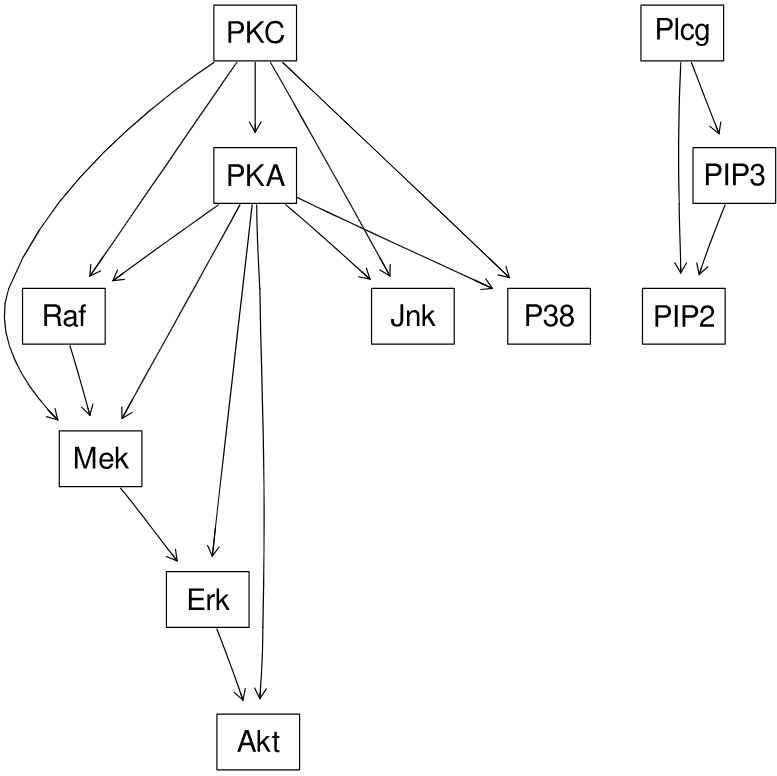
\includegraphics[scale=0.22]{imgs/sachs.png}
			\end{figure}
		\end{column}
	\end{columns}
\end{frame}

\begin{frame}{Examples}
	\begin{itemize}
		\item \textbf{Epidemiology:} Analyzing data on how different treatment or exposures affect health outcomes.
		\item \textbf{Economics and Social Sciences:} Understanding impacts of policy interventions and help in designing potential policies.
		\item \textbf{Machine Learning:} For interpretability, feature selection, making models robust to out of distribution predictions.
	\end{itemize}
\end{frame}

\begin{frame}{Two Main Frameworks}
	Mathematical frameworks for causal inference:
	\vspace{0.5em}
	\begin{itemize}
		\item \textbf{Potential Outcomes Framework} (a.k.a. Rubin's Casual Model)
			\begin{itemize}
				\item Usually interested only in estimating causal effect.
				\item Provides statistical methods for estimating the causal effect.
					Examples are Propensity Score based methods, Doubly robust estimators, etc.
			\end{itemize}
	\end{itemize}
	\vspace{2em}
	\begin{itemize}
		\item \textbf{Directed Acyclic Graphs (DAGs)} / Structural Equation Models (SEMs)
			\begin{itemize}
				\item Causal diagram, i.e., DAG at the core.
				\item The DAG can be used to define estimators for causal effects of interest.
				\item DAGs make modelling assumptions explicit.
			\end{itemize}
	\end{itemize}
\end{frame}

\begin{frame}{Landscape of Causal Inference Python Packages}
	\begin{columns}
		\begin{column}[T]{0.55 \textwidth}
			\center{\textbf{Potential Outcomes Frameworks}}
			\begin{itemize}
				\item Collection of estimation methods
					\begin{figure}
						
\includegraphics[scale=0.2]{imgs/dowhy.png}
					\end{figure}
				\item Doubly Robust Estimation
					\begin{figure}
						
\includegraphics[scale=0.1]{imgs/doubleml.png}
					\end{figure}
				\item Meta Learners: T/S/X-Learners.
					\begin{figure}
						
\includegraphics[scale=0.3]{imgs/causalml.png}
					\end{figure}
			\end{itemize}

		\end{column}
		\vrule
		\begin{column}[T]{0.45 \textwidth}
			\center{\textbf{DAG Frameworks}}
			\begin{itemize}
				\item pgmpy
					\begin{figure}
						
\includegraphics[scale=0.2]{imgs/pgmpy.png}
					\end{figure}
				\item casualnex
					\begin{figure}
						
\includegraphics[height=2cm, width=3cm, scale=0.2]{imgs/causalnex.png}
					\end{figure}
			\end{itemize}
		\end{column}
	\end{columns}
\end{frame}

\begin{frame}{A General Workflow in the DAG Framework}
	\begin{figure}
		\centering
		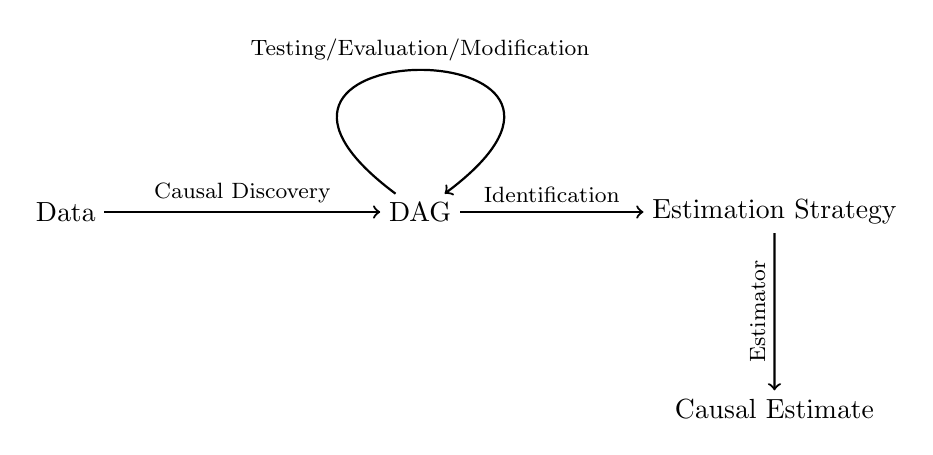
\begin{tikzpicture}[yscale=1, xscale=0.75, inner sep=3pt]
		\tikzstyle{every node}=[align=left]
			\node (data) at (0, 0) {Data};
			\node (dag) at (6, 0) {DAG};
			\node (estimand) at (12, 0) {Estimation Strategy};
			\node (estimation) at (12, -2.5) {Causal Estimate};
	
			\draw[thick, ->] (data) to node[midway, above]{\footnotesize Causal Discovery} (dag);
			\draw[thick, ->] (dag) to node[midway, above] {\footnotesize Identification} (estimand);
			\draw[thick, ->] (estimand) to node[midway, above, rotate=90] {\footnotesize Estimator} (estimation);
			\draw[thick, ->] (dag) [out=150, in=30, looseness=10] to node[midway, above] {\footnotesize Testing/Evaluation/Modification} (dag);
		\end{tikzpicture}
		\label{fig:workflow}
	\end{figure}

	\vspace{1em}

	\center{pgmpy provides functionality to perform each of these steps.}

\end{frame}

% \begin{frame}{What does pgmpy provide}
% 	Will show how to perform each of these steps in pgmpy.
% 	\begin{itemize}
% 		\item Provides standardized implementations of commonly used algorithms.
% 		\item Practical methods methods.
% 		\item Extensible.
% 	\end{itemize}
% \end{frame}

\begin{frame}{Causal Discovery}
	\begin{figure}
		\centering
		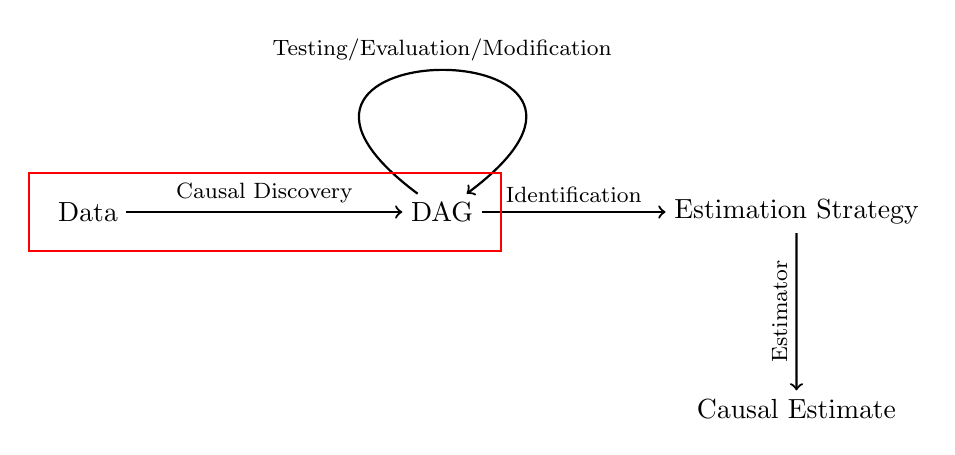
\begin{tikzpicture}[yscale=1, xscale=0.75, inner sep=3pt]
		\tikzstyle{every node}=[align=left]
			\node (data) at (0, 0) {Data};
			\node (dag) at (6, 0) {DAG};
			\node (estimand) at (12, 0) {Estimation Strategy};
			\node (estimation) at (12, -2.5) {Causal Estimate};
	
			\draw[thick, ->] (data) to node[midway, above]{\footnotesize Causal Discovery} (dag);
			\draw[thick, ->] (dag) to node[midway, above] {\footnotesize Identification} (estimand);
			\draw[thick, ->] (estimand) to node[midway, above, rotate=90] {\footnotesize Estimator} (estimation);
			\draw[thick, ->] (dag) [out=150, in=30, looseness=10] to node[midway, above] {\footnotesize Testing/Evaluation/Modification} (dag);

			\draw[draw=red, thick] (-1, -0.5) rectangle (7, 0.5);
		\end{tikzpicture}
		\label{fig:workflow1}
	\end{figure}
	\vspace{1em}
	\center \textbf{Casual Discovery: } Learn the causal DAG from data.
\end{frame}

\begin{frame}{Causal Discovery: Automated Algorithms}
	\begin{itemize}
		\item Many automated algorithms with nice asymptotic properties.
			\begin{itemize}
				\item Constraint-based: PC, Fast Causal Inference.
				\item Score-based: Greedy Equivalence Search, Hill-Climb Search.
				\item Optimization-based: NoTears, DAGMA.
			\end{itemize}
		\item In practice, output varies significantly depending on sample size,
			algorithm used, and their hyperparameters.
		\item With no standard evaluation method, difficult to decide the correct model.
	\end{itemize}
\end{frame}

\begin{frame}{Causal Discovery: Automated Algorithms}
	\begin{figure}
		\begin{subfigure}{0.45 \textwidth}
			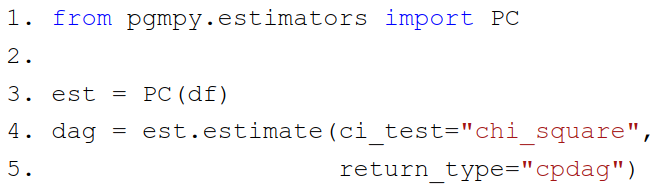
\includegraphics[scale=0.28]{imgs/pc_chisquare.png}
		\end{subfigure}%
		\begin{subfigure}{0.55 \textwidth}
			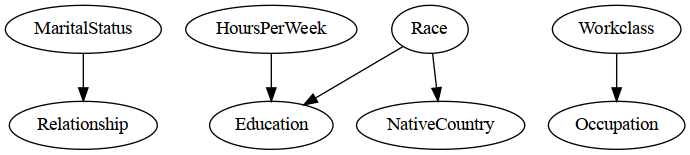
\includegraphics[scale=0.25]{imgs/adult_x2.png}
		\end{subfigure}\vfill
		\begin{subfigure}{0.6 \textwidth}
			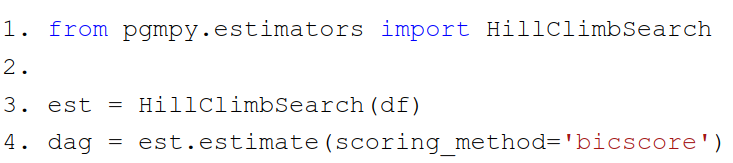
\includegraphics[scale=0.28]{imgs/hill_bic.png}
		\end{subfigure}%
		\begin{subfigure}{0.4 \textwidth}
			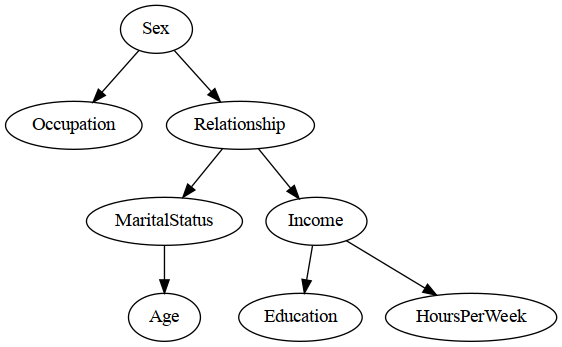
\includegraphics[scale=0.25]{imgs/adult_bic.png}
		\end{subfigure}
	\end{figure}
	\footnotetext{Becker,Barry and Kohavi,Ronny. (1996). Adult. UCI Machine Learning Repository. https://doi.org/10.24432/C5XW20.}
\end{frame}

% \begin{frame}{PC algorithm}
% 	Constraint-Based Algorithm: Exploits Conditional Indpendences in the data to construct the DAG.	
% \end{frame}
% 
% \begin{frame}{Hill-Climb Search}
% 	Score based: Tries to optimize the score by doing local changes.
% 
% 	Results can be very different depending on the algorithm, hyperparameter selections, etc.
% \end{frame}

\begin{frame}{Causal Discovery: Automated Algorithms}
	\begin{figure}
		\begin{subfigure}{0.45\textwidth}
			\centering
			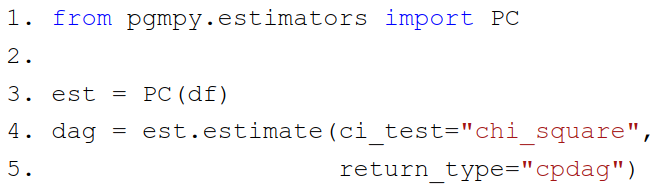
\includegraphics[scale=0.28]{imgs/pc_chisquare.png}
		\end{subfigure}%
		\begin{subfigure}{0.55 \textwidth}
			\centering
			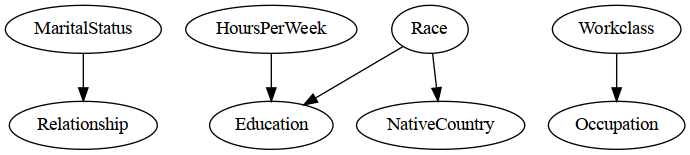
\includegraphics[scale=0.25]{imgs/adult_x2.png}
		\end{subfigure}\vfill
		\begin{subfigure}{0.45 \textwidth}
			\centering
			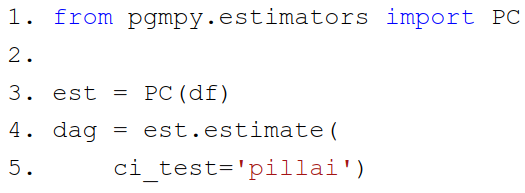
\includegraphics[scale=0.28]{imgs/pc_pillai.png}
		\end{subfigure}%
		\begin{subfigure}{0.55 \textwidth}
			\centering
			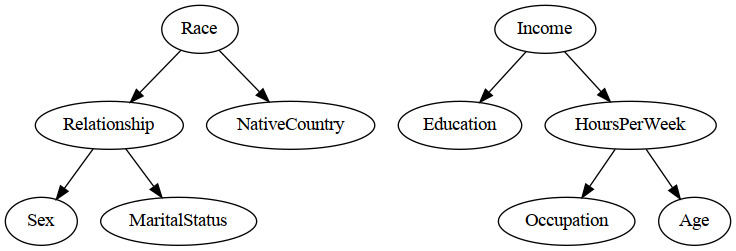
\includegraphics[scale=0.25]{imgs/adult_pillai.png}
		\end{subfigure}
	\end{figure}
\end{frame}

\begin{frame}{Causal Discovery: Problems Automated Algorithms}
	\begin{itemize}
		\item Difficult to choose the best algorithm/model.
		\item In finite sample scenario, all algorithms make mistakes.
		\item Usually requires expert knowlege input.
	\end{itemize}

	\vspace{2em}

	\center{pgmpy implements option to incorporate expert knowledge to these
	algorithms.}
\end{frame}

\begin{frame}{Causal Discovery: Expert Knowledge Integration}
	\begin{itemize}
		\item Users can specify edges to blacklist/whitelist.
		\item The algorithm never adds blacklisted edges and only
			searches over whitelisted edges.
	\end{itemize}
	\vfill
	\begin{figure}
		\begin{subfigure}{0.5 \textwidth}
			\centering
			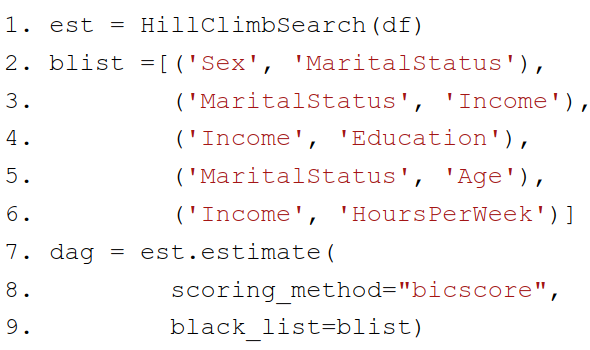
\includegraphics[scale=0.28]{imgs/adult_blacklist.png}
		\end{subfigure}%
		\begin{subfigure}{0.5 \textwidth}
			\centering
			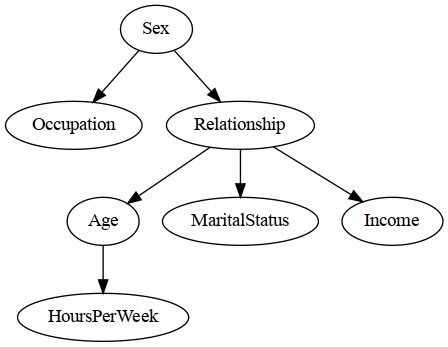
\includegraphics[scale=0.3]{imgs/adult_bic_blacklist.png}
		\end{subfigure}
	\end{figure}
\end{frame}

\begin{frame}{Causal Discovery: Expert Knowledge Integration}
	\begin{itemize}
		\item Score based methods perform local optimization.
	\end{itemize}

	\vfill

	\begin{figure}
		\begin{subfigure}{0.55 \textwidth}
			\centering
			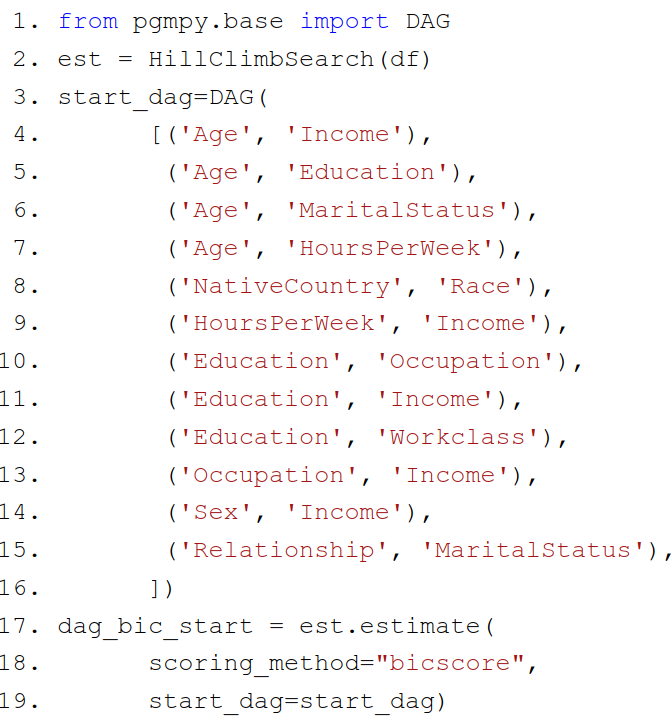
\includegraphics[scale=0.28]{imgs/adult_start.png}
		\end{subfigure}%
		\begin{subfigure}{0.45 \textwidth}
			\centering
			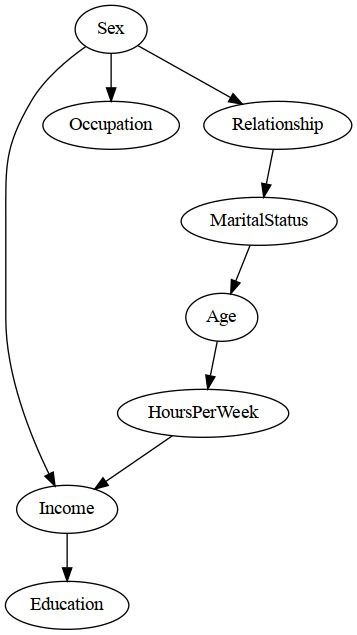
\includegraphics[scale=0.28]{imgs/adult_bic_start.png}
		\end{subfigure}
	\end{figure}
\end{frame}

\begin{frame}{Causal Discovery: Expert Knowledge Integration}
	\begin{itemize}
		\item Allows to specify fixed edges that will be present in the final model.
	\end{itemize}

	\vfill

	\begin{figure}
		\begin{subfigure}{0.5 \textwidth}
			\centering
			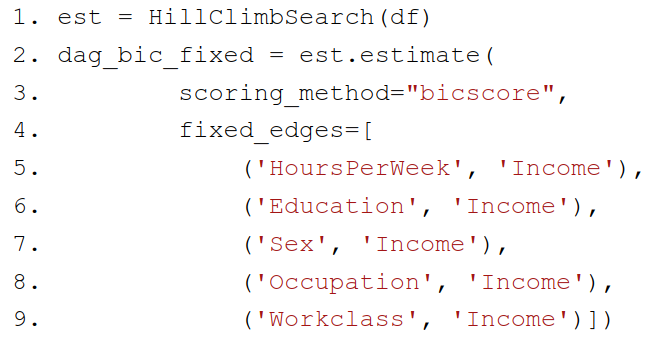
\includegraphics[scale=0.28]{imgs/adult_fixed.png}
		\end{subfigure}%
		\begin{subfigure}{0.5 \textwidth}
			\centering
			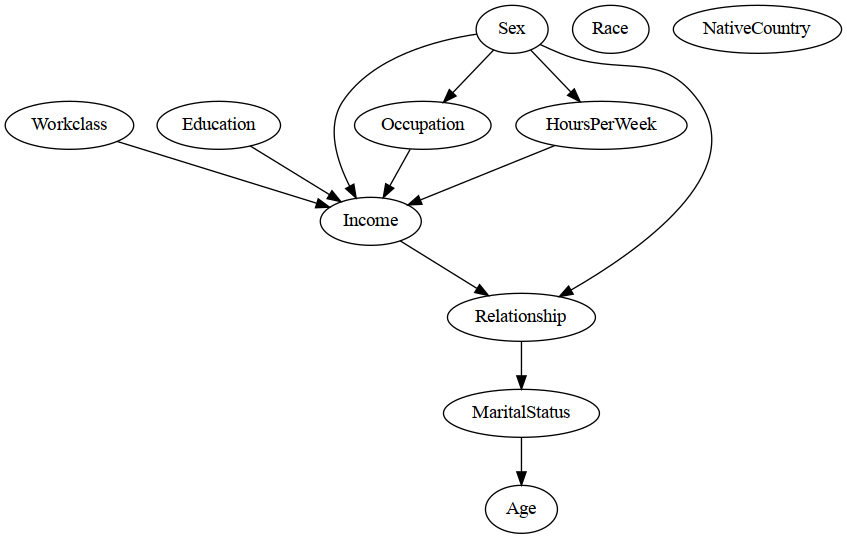
\includegraphics[scale=0.25]{imgs/adult_bic_fixed.png}
		\end{subfigure}
	\end{figure}
\end{frame}

\begin{frame}{Causal Discovery: Expert-In-The-Loop}
	\center{Since, causal discovery in practice is an iterative manual process, we designed an algorithm that works with interactive input from the user.}

	\vspace{2em}

	\begin{itemize}
		\item Finds pair of variables whose observed correlation isn't explained by the model.
		\item Employs a ranking scheme to rank these violations.
		\item Iteratively adds and removes edges.
		\item Uses an expert to decide the direction of the edge.
		\item Greatly reduces the amount of manual intervention required.
	\end{itemize}
\end{frame}
\begin{frame}{Causal Discovery: Expert-In-The-Loop}
	\begin{figure}
		\begin{subfigure}{0.5 \textwidth}
			\centering
			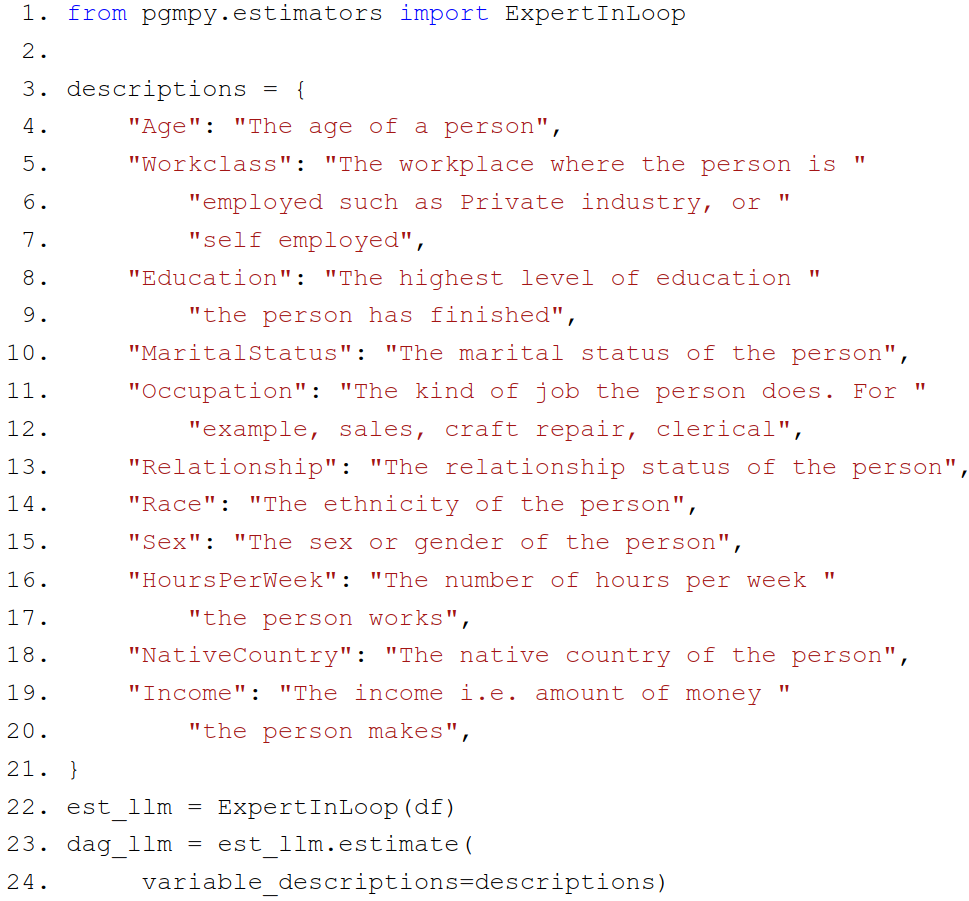
\includegraphics[scale=0.22]{imgs/dag_llm.png}
		\end{subfigure}%
		\begin{subfigure}{0.5 \textwidth}
			\centering
			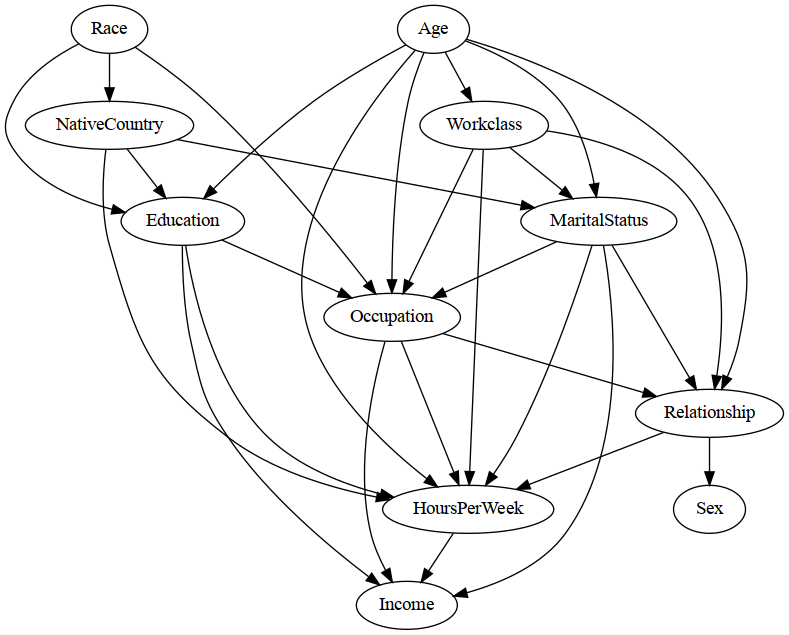
\includegraphics[scale=0.22]{imgs/adult_llm.png}
		\end{subfigure}
	\end{figure}

\end{frame}

% \begin{frame}{Bootstrapping}
% \end{frame}

\begin{frame}{Model Evaluation}
	\begin{figure}
		\centering
		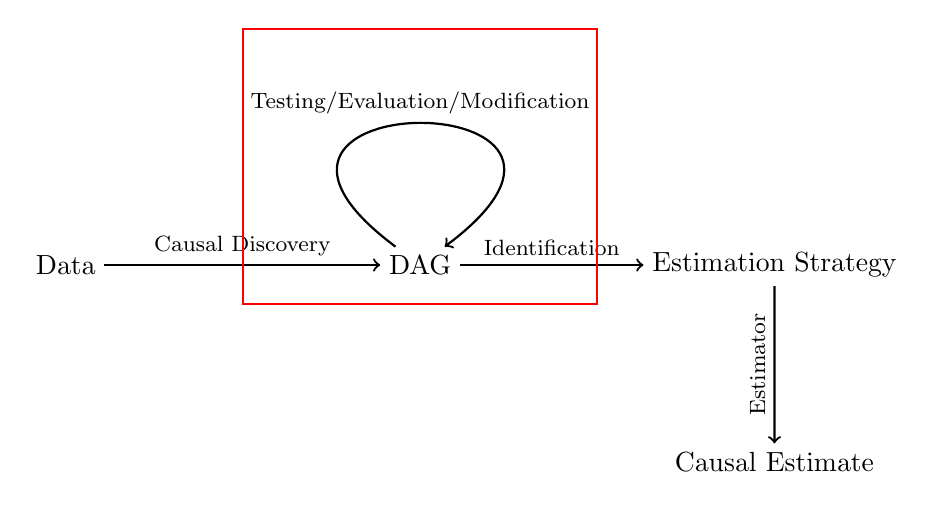
\begin{tikzpicture}[yscale=1, xscale=0.75, inner sep=3pt]
		\tikzstyle{every node}=[align=left]
			\node (data) at (0, 0) {Data};
			\node (dag) at (6, 0) {DAG};
			\node (estimand) at (12, 0) {Estimation Strategy};
			\node (estimation) at (12, -2.5) {Causal Estimate};
	
			\draw[thick, ->] (data) to node[midway, above]{\footnotesize Causal Discovery} (dag);
			\draw[thick, ->] (dag) to node[midway, above] {\footnotesize Identification} (estimand);
			\draw[thick, ->] (estimand) to node[midway, above, rotate=90] {\footnotesize Estimator} (estimation);
			\draw[thick, ->] (dag) [out=150, in=30, looseness=10] to node[midway, above] {\footnotesize Testing/Evaluation/Modification} (dag);

			\draw[draw=red, thick] (3, -0.5) rectangle (9, 3);
		\end{tikzpicture}
		\label{fig:workflow2}
	\end{figure}

	\begin{itemize}
		\item As causal discovery algorithms make mistakes, important to test and modify learned models.
	\end{itemize}
\end{frame}

\begin{frame}{Model Evaluation}
	\center{Similar to unsupervised learning, we do not have any ground truth data, so there is no straightforward way to evaluate models}


	\vspace{2em}

	pgmpy implements a few methods to test and compare models.
\end{frame}

\begin{frame}{Model Evaluation: Implied Conditional Independences (CIs)}
	\begin{figure}
		\centering
		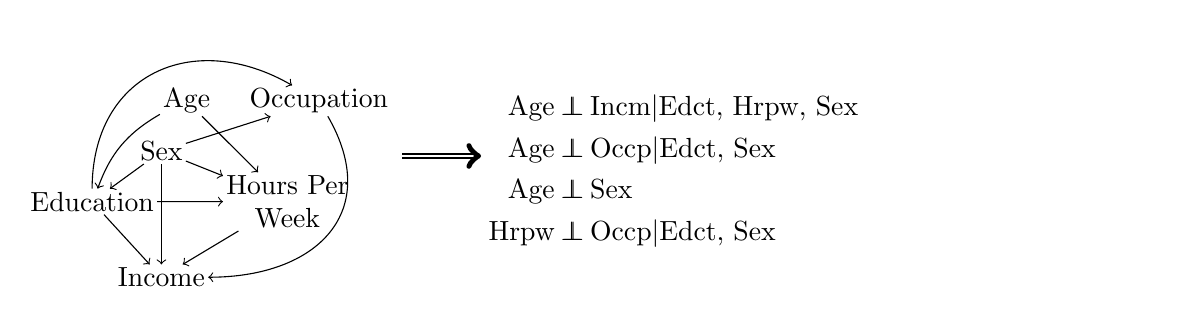
\begin{tikzpicture}
			\begin{scope}[yshift=0.7cm, scale=0.8]
			\tikzstyle{every node}=[align=center, inner sep=1pt]
				\node (sex) at (-0.7, -0.8) {Sex};
				\node (age) at (-0.3, 0) {Age};
				\node (ed) at (-1.8, -1.6) {Education};
				\node (occ) at (1.8, 0) {Occupation};
				\node (hrpw) at (1.3, -1.6) {Hours Per \\ Week};
				\node (income) at (-0.7, -2.8) {Income};
			
				\draw[->]  (age) to[bend right=20] (ed);
				\draw[->]  (sex) to (ed);
				\draw[->]  (age) to (hrpw);
				\draw[->]  (ed) to (hrpw);
				\draw[->]  (sex) to (hrpw);
				\draw[->]  (ed) to (income);
				\draw[->]  (hrpw) to (income);
				\draw[->]  (occ) to[out=300, in=0, looseness=1.4] (income.east);
				\draw[->]  (sex) to (income);
				\draw[->]  (ed) to[out=90, in=150, looseness=1.3] (occ);
				\draw[->]  (sex) to (occ);	
			\end{scope}
			\draw[thick, ->, double] (2.5,0) -- (3.5,0);
			\node[rectangle, align=center, inner sep=1pt] at (6, 0) {
				\begin{minipage}{\textwidth}
					\begin{equation*}
						\begin{split}
							\textnormal{Age} &\ci \textnormal{Incm} \rvert \textnormal{Edct, Hrpw, Sex} \\
							\textnormal{Age} &\ci \textnormal{Occp} \rvert \textnormal{Edct, Sex} \\
							\textnormal{Age} &\ci \textnormal{Sex} \\
							\textnormal{Hrpw} &\ci \textnormal{Occp} \rvert \textnormal{Edct, Sex} \\
						\end{split}
					\end{equation*}
				\end{minipage}
				};
		\end{tikzpicture}
	\end{figure}

	\vspace{2em}
	\begin{itemize}
		\item Each missing edge implies a Conditional Independence (CI).
		\item Statistical tests can be used to check whether they hold in data.
		\item Models can be modified based on these tests.
	\end{itemize}

\end{frame}

\begin{frame}{Model Evaluation: Implied Conditional Independences (CIs)}
	\begin{figure}
		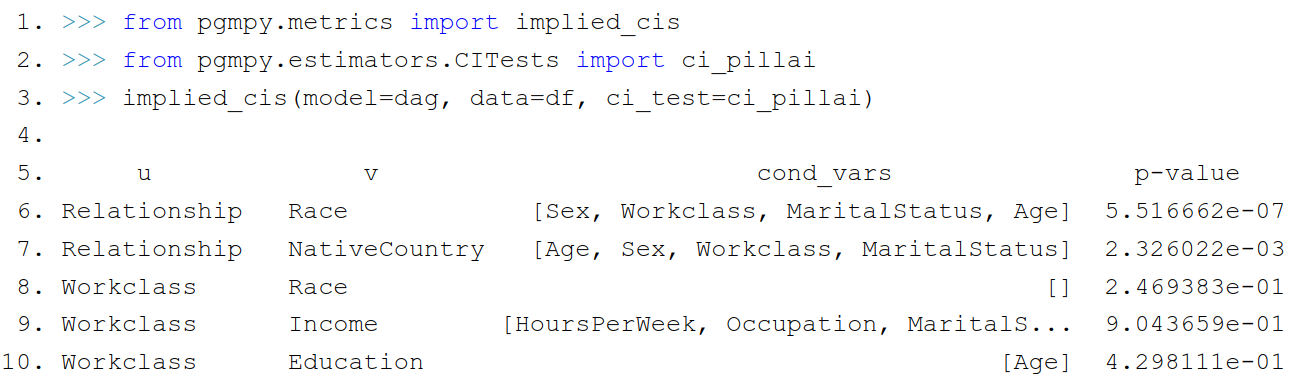
\includegraphics[scale=0.27]{imgs/implied_cis.png}
	\end{figure}
\end{frame}

\begin{frame}{Model Evaluation: Fisher's C Test}
	\begin{itemize}
		\item Combines the implied CI tests to summarize it into a single p-value.
		\item Using some significance threshold, we can decide whether the model fits well to the data.
	\end{itemize}
	\vspace{2em}
	\begin{figure}
		\centering
		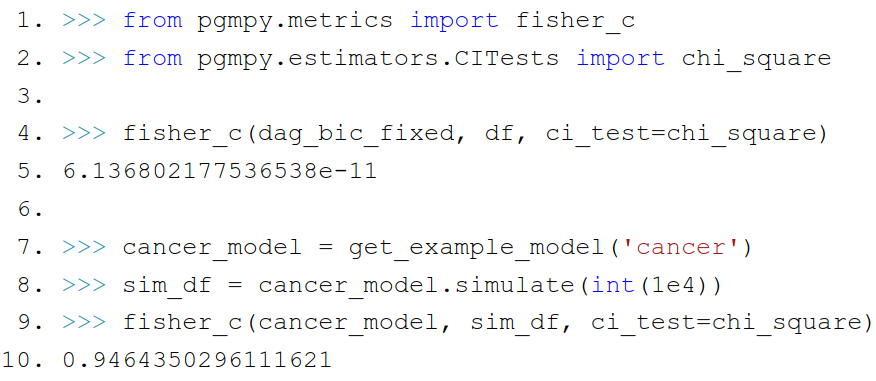
\includegraphics[scale=0.3]{imgs/fisherc.png}
	\end{figure}
\end{frame}

\begin{frame}{Model Evaluation: Correlation Score}
	\begin{itemize}
		\item Compares whether variables that are correlated in data
			are also correlated in the model.
		\item Computes the F1-score based on this comparison.
	\end{itemize}
	\vspace{2em}
	\begin{figure}
		\centering
		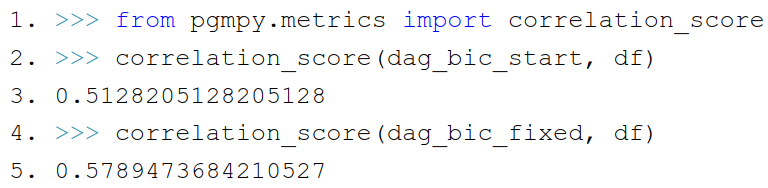
\includegraphics[scale=0.3]{imgs/corr_score.png}
	\end{figure}

\end{frame}


\begin{frame}{Model Evaluation: Structure Score Metrics}
	\begin{itemize}
		\item Scores the network structure based on how well they fit to data.
		\item Useful for comparing multiple models.
	\end{itemize}
	\vspace{1em}
	\begin{figure}
		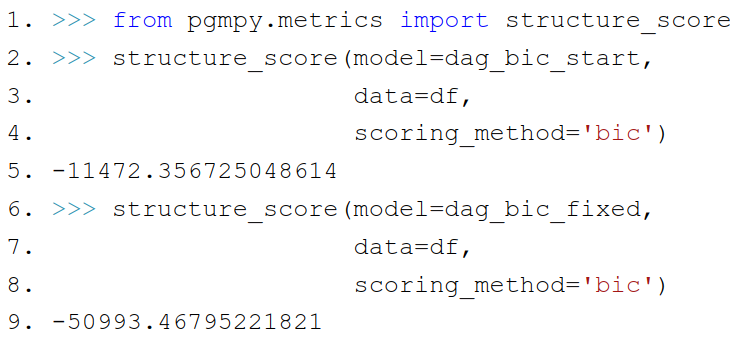
\includegraphics[scale=0.3]{imgs/structure_score.png}
	\end{figure}
\end{frame}

% \begin{frame}{Causal Discovery Algorithms learn a CPDAG}
% 	\begin{figure}
% 	\end{figure}
% 	
% 	\begin{itemize}
% 		\item Trying to learn a network structure which matches the covariance
% 			structure.
% 		\item Multiple networks can represent the same casual structure.
% 		\item Structure learning algorithms usually a DAG.
% 	\end{itemize}
% 
% 	Pairwise edge orientation rules.
% \end{frame}
% 
% \begin{frame}{Minimal Orientation}
% \end{frame}


% \begin{frame}{Using learned DAG in the PO framework}
% 	As DAGs explicitly show all the information, it can be used to make
% 	decisions in the PO framework as well.
% 
% 	The graph can be put into pywhy as well.
% \end{frame}

\begin{frame}{Identification}
	\begin{figure}
		\centering
		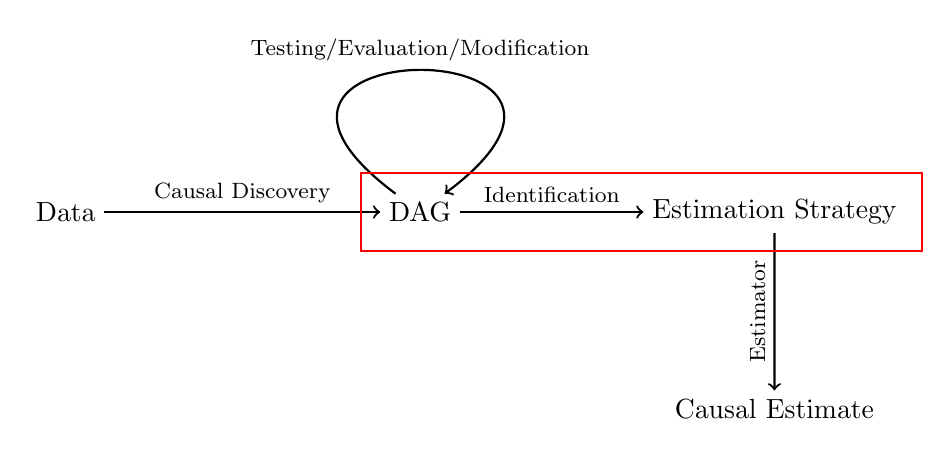
\begin{tikzpicture}[yscale=1, xscale=0.75, inner sep=3pt]
		\tikzstyle{every node}=[align=left]
			\node (data) at (0, 0) {Data};
			\node (dag) at (6, 0) {DAG};
			\node (estimand) at (12, 0) {Estimation Strategy};
			\node (estimation) at (12, -2.5) {Causal Estimate};
	
			\draw[thick, ->] (data) to node[midway, above]{\footnotesize Causal Discovery} (dag);
			\draw[thick, ->] (dag) to node[midway, above] {\footnotesize Identification} (estimand);
			\draw[thick, ->] (estimand) to node[midway, above, rotate=90] {\footnotesize Estimator} (estimation);
			\draw[thick, ->] (dag) [out=150, in=30, looseness=10] to node[midway, above] {\footnotesize Testing/Evaluation/Modification} (dag);

			\draw[draw=red, thick] (5, -0.5) rectangle (14.5, 0.5);
		\end{tikzpicture}
		\label{fig:workflow3}
	\end{figure}
	\begin{itemize}
		\item After decided the DAG, we can start estimating causal effects.
		\item \textbf{Identification}: Is the causal effect of interest estimable?
		\item Everything is identified if all variables are observed.
	\end{itemize}
\end{frame}

\begin{frame}{Identification: do-calculus}
	\begin{figure}
		\begin{subfigure}{0.5 \textwidth}
			\centering
			\includegraphics[page=1]{figures.pdf}
		\end{subfigure}%
		\begin{subfigure}{0.5 \textwidth}
			\centering
			\includegraphics[page=2]{figures.pdf}
		\end{subfigure}
		\label{fig:idnent}
		% \caption{\center{(Left) $ U $ is unobserved; $\beta$ is unidentifiable. (Right) $ U $ is observed; $ \beta $ is identifiable.}}
	\end{figure}

	\begin{itemize}
		\item Theoretically, do-calculus provides a complete solution to identification.
		\item do-calculus can give an estimand for every identified causal effect.
		\item However, no efficient algorithms to get these estimands using do-calculus.
		\item In practice, we rely on a set of simpler identification strategies that work in special cases.
	\end{itemize}
\end{frame}

\begin{frame}{Identification: Backdoor Criterion}
	\begin{itemize}
		\item For cases when biasing paths can be blocked by conditioning.
		\item Finds adjustment variables to block confounding paths.
	\end{itemize}
	\begin{figure}
		\begin{subfigure}{0.5\textwidth}
			\centering
			\includegraphics[page=4]{figures.pdf}
		\end{subfigure}%
		\begin{subfigure}{0.5 \textwidth}
			\begin{equation*}
				\beta_{xy}: Y \sim X + U
			\end{equation*}
		\end{subfigure}
	\end{figure}

	\begin{figure}
		\centering
		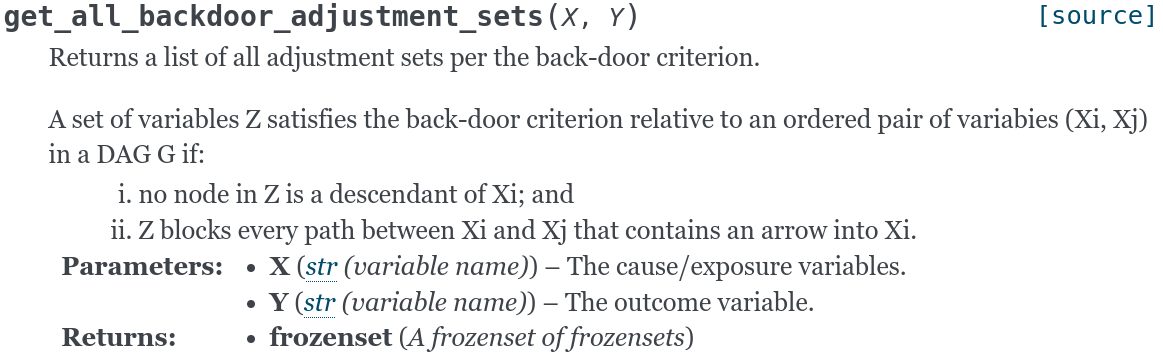
\includegraphics[scale=0.25]{imgs/backdoor.png}
	\end{figure}

\end{frame}

\begin{frame}{Identification: Front-door Criterion}
	\begin{itemize}
		\item Used for scenarios when there are mediator variables.
		\item Double application of backdoor criterion.
	\end{itemize}
	\begin{figure}
		\begin{subfigure}{0.5 \textwidth}
			\centering
			\includegraphics[page=5]{figures.pdf}
		\end{subfigure}%
		\begin{subfigure}{0.5 \textwidth}
			\begin{equation*}
				\begin{split}
					\beta_{xm}:& M \sim X \\
					\beta_{my}:& Y \sim M + X \\
					\beta_{xy} =& \beta_{xm}\beta_{my}
				\end{split}
			\end{equation*}
		\end{subfigure}
	\end{figure}

	\begin{figure}
		\centering
		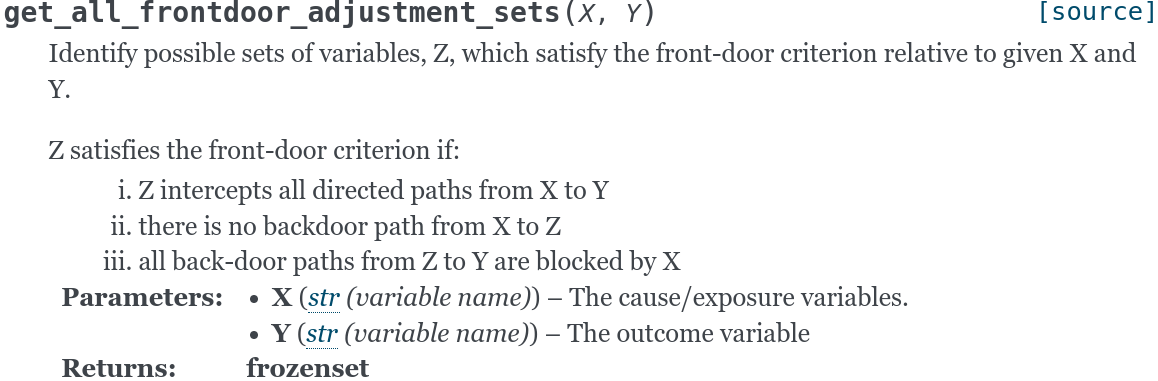
\includegraphics[scale=0.25]{imgs/frontdoor.png}
	\end{figure}
\end{frame}

\begin{frame}{Identification: Instrumental Variables}
	\begin{itemize}
		\item When there are variables in the model that are correlated
			with the outcome variable only through the exposure
			variable.
	\end{itemize}
	\begin{figure}
		\begin{subfigure}{0.5 \textwidth}
			\centering
			\includegraphics[page=6]{figures.pdf}
		\end{subfigure}%
		\begin{subfigure}{0.5 \textwidth}
			\begin{equation*}
				\begin{split}
					\beta_{zx} \beta_{xy}:& Y \sim Z \\
					\beta_{zx}:& X \sim Z \\
					\beta_{xy} =& \frac{\beta_{zx}\beta_{xy}}{\beta_{zx}} \\
				\end{split}
			\end{equation*}
		\end{subfigure}
	\end{figure}

	\begin{figure}
		\centering
		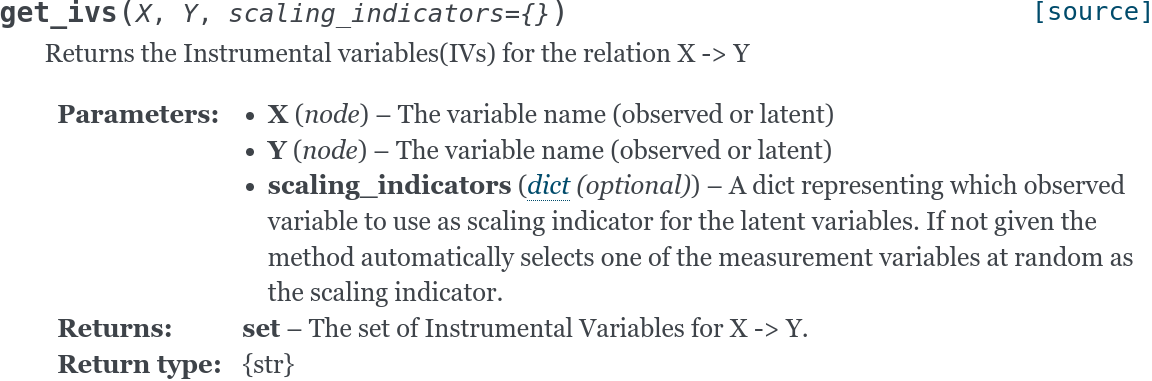
\includegraphics[scale=0.25]{imgs/ivs.png}
	\end{figure}
\end{frame}

\begin{frame}{Estimation}
	\begin{figure}
		\centering
		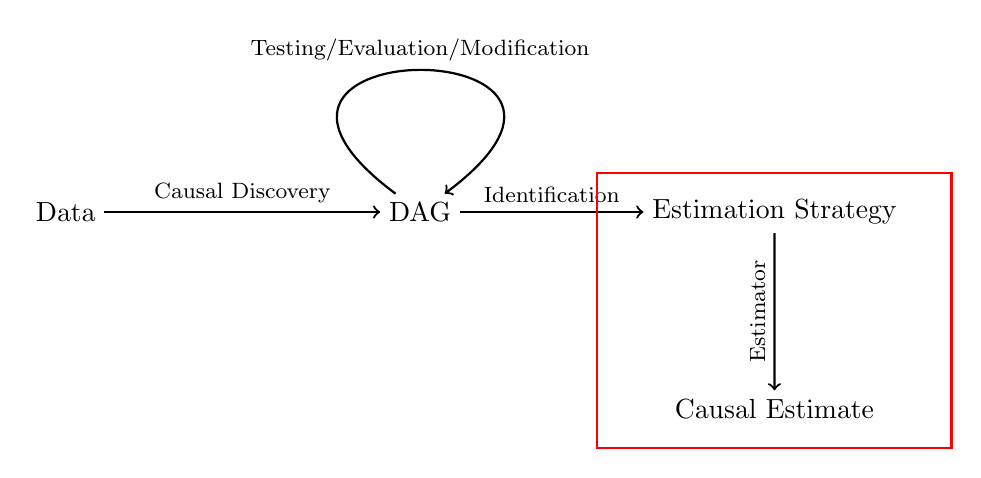
\begin{tikzpicture}[yscale=1, xscale=0.75, inner sep=3pt]
		\tikzstyle{every node}=[align=left]
			\node (data) at (0, 0) {Data};
			\node (dag) at (6, 0) {DAG};
			\node (estimand) at (12, 0) {Estimation Strategy};
			\node (estimation) at (12, -2.5) {Causal Estimate};
	
			\draw[thick, ->] (data) to node[midway, above]{\footnotesize Causal Discovery} (dag);
			\draw[thick, ->] (dag) to node[midway, above] {\footnotesize Identification} (estimand);
			\draw[thick, ->] (estimand) to node[midway, above, rotate=90] {\footnotesize Estimator} (estimation);
			\draw[thick, ->] (dag) [out=150, in=30, looseness=10] to node[midway, above] {\footnotesize Testing/Evaluation/Modification} (dag);

			\draw[draw=red, thick] (9, -3) rectangle (15, 0.5);
		\end{tikzpicture}
		\label{fig:workflow4}
	\end{figure}

	\begin{itemize}
		\item Identification methods give the estimand.
		\item Any estimator can be used to make the estimates.
		\item Usually linear models are used for their interpretability.
	\end{itemize}
\end{frame}

\begin{frame}
	\Huge Some other features.
\end{frame}

\begin{frame}{Simulations}
	\begin{itemize}
		\item Parameterized DAGs are generative models.
		\item Simulated data can be used to evaluate methods.
		\item Can be used for approximate inference.
		\item Helpful in explaining concepts like confounding, bias, etc.
	\end{itemize}
	\begin{figure}
		\centering
		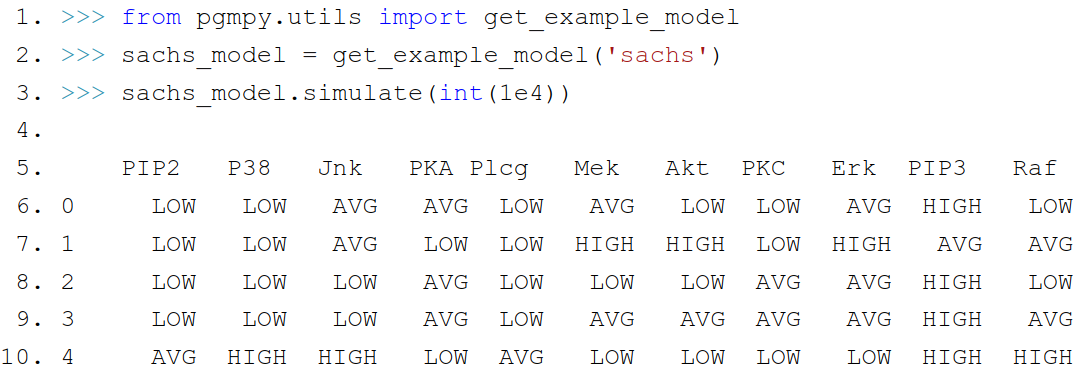
\includegraphics[scale=0.3]{imgs/data_sim.png}
	\end{figure}
\end{frame}
\begin{frame}{Simulations}
	\begin{figure}
		\centering
		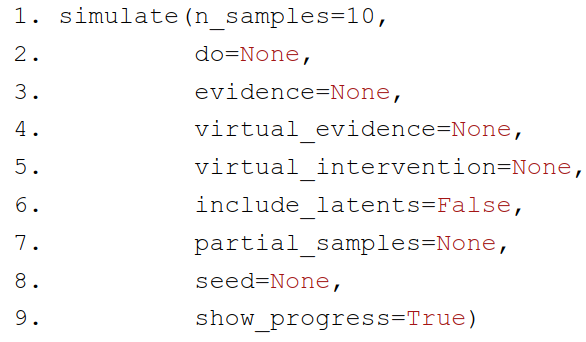
\includegraphics[scale=0.3]{imgs/simulate_fun.png}
	\end{figure}
\end{frame}

\begin{frame}{Extensibility}
	\begin{itemize}
		\item Causal Inference is a very active field of research.
		\item pgmpy offers easy ways to extend/modify algorithms.
		\item Methods accept custom functions as argument.
		\item Base classes make it easier to implement new algorithms and can be plugged into other functionality.
	\end{itemize}
	\vspace{1em}
	\begin{figure}
		\centering
		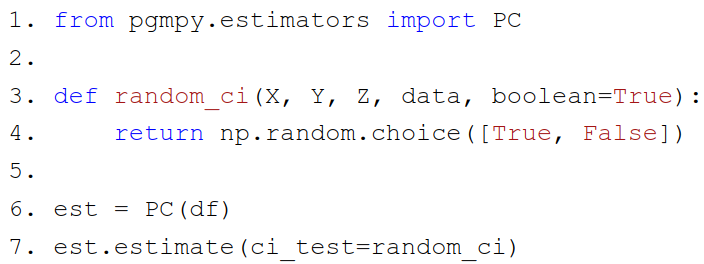
\includegraphics[scale=0.3]{imgs/extend.png}
	\end{figure}
\end{frame}

\begin{frame}{Future Plans}
	\begin{itemize}
		\item Focus on implementing more practical methods such as bootstrapping, model comparison methods.
		\item Improve support for mixed data, i.e., combination of categorical, ordinal, and continuous variables.
		\item Add more commonly used causal discovery, and identification algorithms.
	\end{itemize}
\end{frame}

\begin{frame}
	\center{\Huge {Thank you}}
	\vspace{5em}

	\github : pgmpy/pgmpy
	\vspace{1em}

	\email : ankurankan@gmail.com
\end{frame}

% \begin{frame}{Extra slide}
% 	When to use PO vs DAG framework?
% \end{frame}
% 
% \begin{frame}
% 	How does it compare to Shapley values 
% 	\begin{itemize}
% 		\item Still prediction based. Does not matter if perturbing direct effect variable or undirect.
% 		\item Can show an example where Shapley values would still find an association, but causal inference would not. The standard confounding case.
% 	\end{itemize}
% \end{frame}
\end{document}
